\documentclass[10pt,a4paper]{article}
\usepackage[T1]{fontenc}
\usepackage[utf8]{inputenc}
\usepackage{newtxtext,newtxmath}
\usepackage[scaled=.92]{helvet}
\usepackage[margin=20mm,top=19mm,bottom=20mm]{geometry}
\usepackage{microtype,graphicx,booktabs,array,tabularx,multirow,enumitem}
\usepackage[table]{xcolor}
\usepackage{tikz,pgfplots}
\usetikzlibrary{positioning,arrows.meta,calc}
\pgfplotsset{compat=1.18}
\usepackage[most]{tcolorbox}
\usepackage{fancyhdr,titlesec,hyperref}
\definecolor{ink}{HTML}{152D3A}
\definecolor{teal}{HTML}{167D8D}
\definecolor{gold}{HTML}{C58C36}
\definecolor{rust}{HTML}{B45844}
\definecolor{paper}{HTML}{F1F5F5}
\definecolor{muted}{HTML}{5E6D75}
\definecolor{line}{HTML}{D6E1E3}
\hypersetup{colorlinks=true,linkcolor=teal,urlcolor=teal,pdftitle={Human coding, adjudication and Aperture: a close-reading evaluation},pdfauthor={Codex evaluation with Terra subagent reviews}}
\pagestyle{fancy}\fancyhf{}
\fancyhead[L]{\sffamily\scriptsize\color{muted}APERTURE / ELLIS ISLAND EVALUATION}
\fancyhead[R]{\sffamily\scriptsize\color{muted}06 SEPTEMBER 2026}
\fancyfoot[L]{\sffamily\scriptsize\color{muted}Interpretive audit of supplied artifacts \textbullet\ AI-assisted review}
\fancyfoot[R]{\sffamily\small\color{ink}\thepage}
\renewcommand{\headrulewidth}{0pt}
\setlength{\parindent}{0pt}\setlength{\parskip}{6pt}
\setlength{\emergencystretch}{2em}
\renewcommand{\arraystretch}{1.22}
\setlist[itemize]{leftmargin=14pt,itemsep=3pt,topsep=3pt}
\setlist[enumerate]{leftmargin=17pt,itemsep=4pt,topsep=3pt}
\titleformat{\section}{\sffamily\Large\bfseries\color{ink}}{}{0pt}{}
\titleformat{\subsection}{\sffamily\normalsize\bfseries\color{teal}}{}{0pt}{}
\titlespacing*{\section}{0pt}{0pt}{10pt}
\titlespacing*{\subsection}{0pt}{10pt}{3pt}
\newcolumntype{Y}{>{\raggedright\arraybackslash}X}
\newcommand{\kicker}[1]{{\sffamily\small\bfseries\color{teal}#1}\par\vspace{5pt}}
\newcommand{\source}[1]{{\footnotesize\color{muted}Evidence: #1}\par}
\newcommand{\pill}[2]{\tcbox[on line,colback=#1!12,colframe=#1!12,boxrule=0pt,arc=2pt,boxsep=2pt,left=3pt,right=3pt,top=0pt,bottom=0pt]{\sffamily\scriptsize\bfseries\color{#1}#2}}
\newtcolorbox{takeaway}[1][]{colback=paper,colframe=teal,boxrule=0pt,borderline west={3pt}{0pt}{teal},arc=0pt,left=10pt,right=10pt,top=9pt,bottom=9pt,#1}
\newtcolorbox{caution}[1][]{colback=gold!9,colframe=gold,boxrule=0pt,borderline west={3pt}{0pt}{gold},arc=0pt,left=10pt,right=10pt,top=8pt,bottom=8pt,#1}
\newcommand{\page}[2]{\clearpage\kicker{#1}\section*{#2}}
\newcommand{\case}[4]{\subsection*{#1}\textbf{Human / adjudication.} #2\par\textbf{AI / assessment.} #3\par\source{#4}}
\begin{document}
\thispagestyle{empty}
\vspace*{7mm}
\kicker{RESEARCH EVALUATION \hfill 06 SEPTEMBER 2026}
{\sffamily\fontsize{34}{38}\selectfont\bfseries\color{ink}Human coding,\\adjudication\\and Aperture\par}
\vspace{5mm}
{\Large\color{muted}What changes when we read the meanings,\\rather than count matching labels?\par}
\vspace{10mm}

\begin{tikzpicture}
\fill[ink] (0,0) rectangle (17,2.25);
\node[anchor=west,text=white] at (.55,1.45) {\sffamily\LARGE\bfseries 8 interviews};
\node[anchor=west,text=white] at (6.1,1.45) {\sffamily\LARGE\bfseries 3 human coders};
\node[anchor=west,text=white] at (12.1,1.45) {\sffamily\LARGE\bfseries 1 AI export};
\node[anchor=west,text=white!75] at (.55,.65) {\small Ellis Island oral histories};
\node[anchor=west,text=white!75] at (6.1,.65) {\small Individual work + calibration};
\node[anchor=west,text=white!75] at (12.1,.65) {\small 985 claims / 28 evidenced themes};
\end{tikzpicture}
\vspace{7mm}
\begin{takeaway}
\textbf{Overall finding.} Aperture offers substantial interpretive overlap with the human work and useful alternative readings. The strongest human contribution is explicit discussion of analytical boundaries and long-term meaning. Both sides sometimes move beyond their evidence. The calibration record is a valuable comparator, but it is not a verified answer key.
\end{takeaway}
\vspace{3mm}
\textbf{Three conclusions replace the package's headline comparison.}
\begin{enumerate}
\item \textbf{The ``near-zero agreement'' claim is not supported.} Many differently named human codes express the same meaning; unique selection is not disagreement. The session itself repeatedly recognises conceptual convergence.
\item \textbf{The AI does interpret and synthesise.} It lacks a named overarching-theme tier, but its corpus narrative relates adult migration infrastructure to partial childhood memory. Its weaker point is integration of long-term, intergenerational consequences.
\item \textbf{Agreement can preserve an error.} The session misidentifies Batta's religion. Her interview explicitly says Roman Catholic; the AI's cross-ethnic reading is better supported in that case.
\end{enumerate}
\vfill
{\small\color{muted}Prepared through close reading of the supplied evaluation package, with Terra subagents assigned to transcript evidence and the lead reviewer responsible for adjudication, thematic synthesis and source checks. This is an AI-assisted interpretive audit, not an independently human-validated benchmark. The accompanying ledger makes the judgments contestable.}

\page{01 / EVALUATION STRATEGY}{Compare reasoning at the same level}
\begin{takeaway}
\textbf{Evaluation question.} Which meanings do the individual coders, their calibration process and Aperture preserve, add, flatten or overstate, and how well do those meanings explain the interview evidence?
\end{takeaway}
\subsection*{Three comparisons, not a single agreement score}
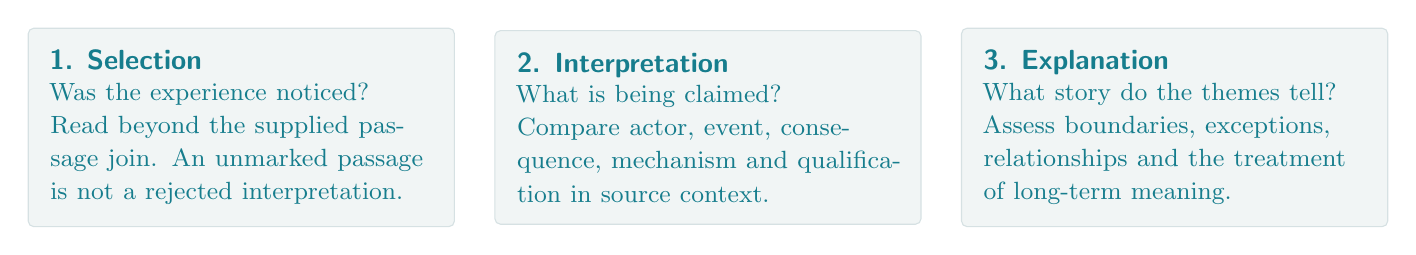
\begin{tikzpicture}[node distance=5mm,box/.style={draw=line,fill=paper,rounded corners=2pt,text width=4.85cm,minimum height=2.35cm,align=left,inner sep=8pt},>=Latex]
\node[box] (a) {\sffamily\bfseries\color{teal}1. Selection\par\normalfont\small Was the experience noticed?\par Read beyond the supplied passage join. An unmarked passage is not a rejected interpretation.};
\node[box,right=of a] (b) {\sffamily\bfseries\color{teal}2. Interpretation\par\normalfont\small What is being claimed?\par Compare actor, event, consequence, mechanism and qualification in source context.};
\node[box,right=of b] (c) {\sffamily\bfseries\color{teal}3. Explanation\par\normalfont\small What story do the themes tell?\par Assess boundaries, exceptions, relationships and the treatment of long-term meaning.};
\end{tikzpicture}
\subsection*{The unit is a defensible meaning in context}
A human code can span several sentences; an AI claim often paraphrases a short fragment. We therefore treat each of the 267 consolidated rows as an \emph{evidence dossier}, not as one interchangeable code. The three human readings form a set of possible interpretations. A majority does not automatically establish truth, and agreement with one coder need not preserve every other coder's insight.

For each dossier the passage reviewers read the human labels and explanatory notes, the interview, and the AI claims for that interview. They consider claims beyond the lexical join. ``Same event'' is weaker than ``same meaning'': an AI description of a detention procedure may still miss the human reading of uncertainty, humiliation or solidarity.

\begin{tabularx}{\linewidth}{@{}p{3.6cm}Y@{}}
\toprule
\textbf{Judgment} & \textbf{Decision rule}\tabularnewline\midrule
Substantive match & The AI captures the central supported human meaning; different wording or theme placement is acceptable.\tabularnewline
Partial / different lens & The experience is shared, but a consequential human meaning is absent, narrower, or reframed.\tabularnewline
Human insight missing & No equivalent AI interpretation was located after reading the transcript's complete claim set.\tabularnewline
Unsupported human inference & The human interpretation materially exceeds the available source; use separately from supported readings on that row.\tabularnewline
Unresolved & The available evidence or provenance cannot sustain a confident comparison.\tabularnewline\bottomrule
\end{tabularx}
\subsection*{What makes an interpretation stronger?}
Four criteria guide the final judgment: \textbf{fidelity} to what was said and who said it; \textbf{analytic value} beyond retelling; \textbf{coherence} within and between themes; and \textbf{calibration}, including qualifiers, counterexamples and open questions. These are argued judgments, not numerical grades.

The methodological choice fits the authors' distinction between reflexive thematic analysis and coding-reliability approaches: coding consensus is not itself a test of analytic quality. A theme also needs an organising meaning, rather than only a shared topic. See Braun and Clarke's \href{https://www.thematicanalysis.net/faqs/}{methodological FAQ} and \href{https://www.thematicanalysis.net/editor-checklist/}{reviewer guidance}.
\source{Crosswalk rows 1--267; original human books; T1--T8; machine claims and narratives. The rules above are this evaluation's protocol, not rules supplied by the original coders.}

\page{02 / PACKAGE AUDIT}{What the counts can actually tell us}
\begin{tabularx}{\linewidth}{@{}Yrrrr@{}}
\toprule
 & \textbf{C1} & \textbf{C2} & \textbf{C3} & \textbf{Aperture}\tabularnewline\midrule
Initial rows / claims & 193 & 159 & 107 & 985\tabularnewline
Final candidate-theme labels & 9 & 5 & 7 & 31\tabularnewline
Themes with claim evidence & --- & --- & --- & 28\tabularnewline
Named overarching themes & 4 & 2 & 2 & 0\tabularnewline\bottomrule
\end{tabularx}
{\footnotesize\color{muted}Human counts describe workbook rows, some containing multiple codes. C1's earlier pass adds three labels, not three more final themes. C2's final overarching sheet contains two themes; earlier drafts are not additional findings.}

\subsection*{Human selection is sparse relative to the union of selections}

\begin{tikzpicture}
\fill[teal] (0,0) rectangle (7.70,.75);
\fill[gold] (7.70,0) rectangle (14.13,.75);
\fill[ink] (14.13,0) rectangle (17,.75);
\node[text=white,font=\sffamily\bfseries] at (3.85,.375) {121 / one coder};
\node[text=white,font=\sffamily\bfseries] at (10.92,.375) {101 / two coders};
\node[text=white,font=\sffamily\bfseries] at (15.565,.375) {45 / three};
\end{tikzpicture}
{\footnotesize\color{muted}Figure 1. Number of occupied coder cells in each consolidated row, $n=267$. This is selection overlap, not interpretive agreement.}

The consolidated book assigns 121 rows to ``Divergence,'' 121 to ``Unique coding,'' 24 to partial convergence and one to strong convergence. These labels reproduce its taxonomy; they do not establish that the humans agreed on only one meaning. Of the 267 rows, 121 were selected by just one coder. The remaining 146 are still neither fixed coding opportunities nor independent observations for a reliability statistic.

\begin{caution}
\textbf{78\% is passage retrieval, not AI accuracy.} The lexical crosswalk links 208 of 267 human rows to at least one AI claim. Its 59 unlinked rows need reading. Conversely, a linked claim may capture only a minor detail of the passage. The 570 unaligned AI claims are candidates for review, not 570 novel discoveries.
\end{caution}
\subsection*{Density and self-checking need qualification}
The 985 AI claims rest on 797 distinct transcript--passage pairs. Multiple claims may concern the same episode, and shared passages appear under more than one theme. Greater output volume establishes greater elaboration, not greater sensitivity or quality.

There are \textbf{371 caveated claims} (37.7\%). Some caveats concern support from an adjacent passage or an added analytical term; others identify more consequential inferential gaps. Neither the presence nor absence of a caveat establishes correctness. Four theme/material summaries explicitly flag overreach, while the corpus processing log contains additional exclusions and warnings. The four are not an exhaustive error count.

The export records 68 theme/material pairs as ``not looked for here'' and five as ``found too thin.'' Single-material themes must therefore be read as locally developed findings, not proven corpus-unique patterns. Three empty themes are placeholders.

\textbf{Workflow fairness.} This is one exported AI analysis, not a one-call experiment: its processing history lists multiple reading, theme-development, comparison, checking and rewriting stages. Human coders also describe recursion and earlier calibration. There is no matched time, cost or iteration budget, and no basis for an efficiency ranking.
\source{Package JSON counts independently checked; \texttt{package\_stats.json} and \texttt{input\_manifest.json} accompany the report. Raw Excel/Word extraction fidelity was asserted by the preparer and was not re-audited here.}

\page{03 / WHAT ADJUDICATION DISCOVERED}{Convergence in meaning; disagreement in structure}
\begin{tabularx}{\linewidth}{@{}p{3.3cm}Yp{3.9cm}@{}}
\toprule
\textbf{Issue} & \textbf{What the session establishes} & \textbf{Implication for AI comparison}\tabularnewline\midrule
Different code labels & Voyage sickness, Scottish traditions and homesickness are explicitly recognised as shared meanings. The group describes stronger initial-code convergence than divergence. & Exact label agreement is the wrong baseline. Retain meaningful differences in scope.\tabularnewline
Delayed reunion & ``Family separation'' is preferred as the primary meaning of T1's long wait. Money or visa explanations are not specified in that extract. & Reward restraint about causal explanations, but inspect surrounding context before rejecting a broader reading.\tabularnewline
Family versus community & C3 recognises that family reunion was placed under community partly because she did not know where else to put it. The group accepts distinguishing the concepts. & Test whether kin resources and co-ethnic belonging remain analytically distinguishable.\tabularnewline
Theme splitting & Arrival emotions are separated from adaptation; work/education may be separated from perseverance; pre-migration circumstances, possibilities and hopes may be split. & These are boundary proposals and some accepted distinctions, not a fully revised consensus codebook.\tabularnewline
Overarching structure & C1 preserves four dimensions; C2 compresses into departure/cost and settlement; C3 combines practical transition with identity/belonging. & Compare explanatory functions, not whether the AI reproduces a four-theme tree.\tabularnewline
Analytic constraints & Coders discuss a seven/eight candidate-theme expectation, a perceived two/three overarching-theme limit, prior theory and the absence of a focused research question. & The human--AI granularity difference is partly a task-design difference.\tabularnewline\bottomrule
\end{tabularx}

\subsection*{Adjudication is not the same as a final reference standard}
The meeting selects examples and discusses alternative structures. It does not recode all 267 rows in sequence or agree one final thematic hierarchy. C3 continues to defend a broad ``barrier'' interpretation after the family-separation discussion. At the end, C1 says she will compile the books. The consolidated 9+4 patterns are useful comparison dimensions, but their existence does not prove ratification of a single shared analysis.

\begin{takeaway}
\textbf{What should travel into the evaluation?} The calibration's reasons: preserve the main phenomenon; distinguish family from community; allow multiple meanings within one extract; and keep a theme's organising idea clear. Its consensus statements must still be tested against the interviews.
\end{takeaway}
\source{Calibration session lines 9--98 (sickness), 257--307 (traditions/homesickness), 308--526 and 1613--1692 (separation), 908--1041 (family/community), 784--907 and 1090--1152 (splits), 1153--1249 and 1296--1432 (constraints/structure), closing turns at 1:20:41--1:20:52. Line references follow the package's verbatim Markdown.}

\page{04 / ADJUDICATION UNDER TEST}{A settled interpretation can still be wrong}
\kicker{CASE A / BATTA'S RELIGION}
\begin{tabularx}{\linewidth}{@{}YY@{}}
\toprule
\textbf{Calibration account} & \textbf{Interview evidence}\tabularnewline\midrule
C3 asks whether the Hungarian participant was Catholic rather than Jewish. C1 insists she was from a Jewish community; C3 accepts the correction. The package index presents this as a factual correction. & Asked what religion she was, Batta answers ``I was a Catholic'' and then ``Roman Catholic.'' Later she describes Jewish friends in her place of origin and using the Jewish kitchen at Ellis Island.\tabularnewline\bottomrule
\end{tabularx}

\textbf{Why it matters analytically.} Shared religious identity would support an interpretation of maintaining one's own religious community. The actual evidence supports a Catholic participant drawing on cross-community familiarity and relationships. These are different mechanisms of settlement and assistance. ``Where I came from there's plenty Jewish people'' does not make the narrator Jewish.

\textbf{How the AI stacks up.} Aperture's detention narrative reads this episode as cross-ethnic solidarity; its claims refer to familiarity and friendship with Jewish people. That is better supported than the meeting's identity inference. This is a local evidentiary advantage, not proof that AI adjudication is generally superior.
\source{T7 source lines 169--183 and 329--331; calibration lines 227--256; crosswalk row 220; machine theme ``Navigating immigration detention,'' T7 passages S328--S329.}

\vspace{4mm}
\kicker{CASE B / THE LIMITS OF CAUSAL INFERENCE}
In T1, a father leaves first and his family follows seven or eight years later. C1 and C2 code separation; C3 codes immigration-process barriers. The session usefully asks which mechanism is actually evidenced. C3 acknowledges thinking of money or visas, while maintaining that a delay implies some obstacle.

The most defensible resolution is to separate \textbf{the observed relation} (prolonged separation) from \textbf{a plausible explanation} (barriers of unspecified kind). The later Warsaw paperwork wait supplies evidence of a particular delay; it does not by itself explain the entire preceding interval. Aperture captures the separation and leaves causes as an open question.
\source{T1 source paragraph beginning ``I think she made it'' and later Warsaw account; crosswalk rows 1 and 6; calibration lines 308--526, 1613--1692; AI T1 ``Family separation'' S055/S057 and corpus open questions.}

\begin{caution}
\textbf{Process caution.} The session repeatedly seeks assent, and the religion case shows assent surviving a source contradiction. That does not establish motives or a general social-pressure effect. It does justify checking the evidence behind agreement. The ASR transcript also contains speaker/pronoun confusion, so factual claims should be traced to the interview rather than inferred from fluent meeting summaries.
\end{caution}

\page{05 / THE INDIVIDUAL HUMAN READINGS}{Different analytic ambitions, different risks}
\begin{tabularx}{\linewidth}{@{}p{2.7cm}YY@{}}
\toprule
\textbf{Coder} & \textbf{Contribution visible in the books} & \textbf{Risk visible in the books}\tabularnewline\midrule
\textbf{C1 / Nirosha}\newline193 initial rows; 9 final candidates; 4 overarching themes & Most differentiated final architecture. Separates relational resources, participation/rebuilding and retrospective meaning. Memos ask whether support enables wider participation or preserves boundaries. & A network can be treated as a source of security without sufficient evidence of felt belonging. The calibration's Batta example imports shared identity incorrectly.\tabularnewline
\textbf{C2 / Arnisha}\newline159 initial rows; 5 candidates; 2 final overarching themes & Expressive interpretation of embodied hardship, family survival, uneven settlement and intergenerational outcomes. Explicitly connects empirical readings to theory. & Broad titles and theoretical classifications can outrun their evidence. ``Leaving costs everything'' risks flattening comfortable origins or positive experiences. Assigning whole-life acculturation categories is stronger than documenting a particular schooling or cultural episode.\tabularnewline
\textbf{C3 / Karolina}\newline107 initial rows; 7 candidates; 2 overarching themes & Often concrete distinctions: language, identity/discrimination, arrival reactions. Recognises mixed arrival emotions and the need to revise earlier groupings. & Broad ``challenges'' can combine distinct causes and stages. Pre-migration drivers and long-term/intergenerational meaning are not independently developed; family reunion is initially absorbed into community.\tabularnewline\bottomrule
\end{tabularx}

\subsection*{Interpretive depth is not the same as theoretical certainty}
C2's final overarching sheet calls Kaiz's experience closer to marginalisation and describes her as belonging fully to neither world. The interview directly supports educational disruption, a perceived lack of study skills and lasting regret. It does not establish that comprehensive identity diagnosis. Similarly, a narrative comparison of two families cannot isolate resources and reception as the determinants of their different life courses.

C1's reflections are often more carefully framed as questions: how do resources support participation and maintain boundaries, and can later gains coexist with earlier losses? Those questions create analytic depth without requiring a causal conclusion the interviews cannot establish. C3's more descriptive architecture can be less explanatory, but description is not automatically inferior when the evidence is thin.

\subsection*{The AI offers a fourth lens}
The AI's strongest additional organising ideas concern \textbf{memory and mediation}, \textbf{property and relative class position}, and \textbf{the social limits of enclaves}. These do not simply reproduce the humans' migration-stage structure. They can enrich it, provided their mechanisms are qualified and their exceptions retained. Novelty must be judged relative to the whole human record: for example, C1 already reflects on communities preserving boundaries, so that AI lens is not wholly human-absent.

\source{Original human candidate/overarching sheets, with continuation rows read together; C2's final sheet ``Overarching themes''; T1 source line 152; consolidated coder-theme details; calibration lines 1296--1432 and 1966--2049. This table characterises these artifacts, not coder ability in general.}

\page{06 / CANDIDATE PATTERNS, 1--5}{Where Aperture carries the human analysis}
{\small These are the consolidated book's comparison dimensions. Correspondence is judged from definitions, supporting claims and narrative logic, not matching titles.}\par
\begin{tabularx}{\linewidth}{@{}p{3.4cm}YY@{}}
\toprule
\textbf{Human pattern} & \textbf{AI correspondence} & \textbf{Close-reading assessment}\tabularnewline\midrule
\textbf{1. Pre-migration constraint, danger and imagined possibility} & Violence as habitual backdrop; economic push/pull; property as economic foundation. & \textbf{Strong but differently organised.} The AI separates persecution, economic motivation and relative comfort. This answers the session's concern about collapsing danger and aspiration. Property and comfortable origins supply useful counterexamples to a universal deprivation narrative.\tabularnewline\addlinespace
\textbf{2. Hardship, uncertainty and institutional control} & Child's threshold; detention; violence; local freedom/ordeal and theft themes. & \textbf{Substantial, with uneven bodily coverage.} The AI explains sorting, separation, disguise and political intervention. It distributes journey experience across narrower themes; some human accounts of bodily suffering remain less explicit. An empty ``Migration journey'' placeholder does not mean the entire subject is absent.\tabularnewline\addlinespace
\textbf{3. Family as a resource} & Known contacts; family separation/reunion; household authority; property. & \textbf{Strong mechanism-level correspondence.} Money, paperwork, destinations and care become an account of migration infrastructure. Family and enclave are distinguishable, addressing a calibration concern. The AI also retains relatives who could not help as a counterexample.\tabularnewline\addlinespace
\textbf{4. Separation, loss and attachment} & Family separation/reunion; emotional weight of homeland/migration; partial/mediated memory. & \textbf{Strong, including ambivalence.} Refused reunion, unreturned parents, continuing attachment and explicit disavowal of regret complicate a simple reunion-success story. The emotional theme's breadth sometimes weakens its boundary.\tabularnewline\addlinespace
\textbf{5. Expectations and arrival} & Child's threshold; economic push/pull; emotional weight; local educational-promise theme. & \textbf{Strong contrast, dispersed structure.} Wonder, fear, disappointment and institutional vulnerability are present. The AI's child/adult perspective can add explanatory value, but ``both at once'' should not imply every narrator experienced the same mixed response.\tabularnewline\bottomrule
\end{tabularx}

\begin{takeaway}
\textbf{The relevant question is preservation, not tree shape.} An AI theme can serve several human comparison dimensions. Conversely, several AI themes may jointly preserve a human pattern. Neither relationship should be forced into a one-to-one label crosswalk.
\end{takeaway}
\source{Consolidated candidate-pattern rows 1--5; machine theme definitions and complete cross-material narratives; local theme/material summaries; calibration discussion of pre-migration splitting and family/community distinction.}

\page{07 / CANDIDATE PATTERNS, 6--9}{Where the human synthesis remains stronger}
\begin{tabularx}{\linewidth}{@{}p{3.4cm}YY@{}}
\toprule
\textbf{Human pattern} & \textbf{AI correspondence} & \textbf{Close-reading assessment}\tabularnewline\midrule
\textbf{6. Community, continuity, support and belonging} & Bounded enclave; known contacts; heritage language; ethnic institutions formed/fading. & \textbf{Rich complementary lens.} The AI examines both support and confinement, and institutional decline. The human distinction between resources and felt belonging remains valuable. The AI should not infer that neighbourhood residence itself proves either insularity or exclusion.\tabularnewline\addlinespace
\textbf{7. Language, difference, identity and participation} & Language as barrier/gateway; language practices; bounded enclave; religious observance. & \textbf{Strong on language; less integrated on discrimination.} The barrier/practice split distinguishes institutional access from learning mechanisms. Human codes more explicitly preserve identity pressure, social exclusion and discrimination in some episodes. These may be lost when the AI centres language acquisition alone.\tabularnewline\addlinespace
\textbf{8. Education, work and perseverance} & Local themes on class descent, displaced craft, women's work, household labour, rental economy and workplace freedom. & \textbf{Detailed, but dispersed.} The AI gives concrete trajectories and mechanisms rather than one generic adaptation theme. C1/C2 more explicitly connect these to the ongoing project of rebuilding life. ``Perseverance'' is useful only when it adds to the observed work and constraints.\tabularnewline\addlinespace
\textbf{9. Long-term / intergenerational meaning} & Emotional weight; class descent/education; failed educational promise; later volunteerism; heritage language and institutional decline. & \textbf{Present in pieces; weaker as a governing explanation.} The AI notices regret, justified suffering and descendants' gains. C1 and C2 more clearly organise how later lives change the meaning of earlier sacrifice. C3 also has no standalone equivalent, so this is not a unanimous human advantage.\tabularnewline\bottomrule
\end{tabularx}

\subsection*{A productive disagreement: cultural continuity or bounded participation?}
The human community themes emphasise familiarity, help and continuity. The AI's enclave narrative asks what happens when that familiar world meets school and employment. It can explain why children gain new social opportunities while adults continue using the heritage language. It also includes mixed neighbourhoods, class exclusion inside an ethnic community and a Danish case of rapid English learning.

The danger is turning those cases into a universal causal sequence in which employment necessarily ``breaks'' the enclave. The narrative's own counterexamples require a qualified formulation: \emph{in some accounts, school or work broadened contact beyond the ethnic neighbourhood; maintaining cultural ties and widening participation could coexist.}

\source{Consolidated candidate-pattern rows 6--9; AI ``Ethnic enclave,'' both language themes, and local economic/work themes; C1 final candidate and overarching reflections; C2 final overarching narrative.}

\page{08 / OVERARCHING INTERPRETATION}{The AI has synthesis, but a different centre}
\begin{takeaway}
\textbf{Artifact-level absence is real; interpretive absence is not.} The export has no field containing named overarching themes. Yet \texttt{what\_this\_may\_mean} proposes a corpus interpretation linking adult infrastructure to the fragments children retained. That is a higher-order analytical move and should be evaluated on its substance.
\end{takeaway}
\begin{tabularx}{\linewidth}{@{}p{4.3cm}Y@{}}
\toprule
\textbf{Consolidated overarching dimension} & \textbf{How the AI compares}\tabularnewline\midrule
1. Conditions, disruption and the migration process & Functionally present: violence, economic differentiation, contacts, institutional encounters and fragmented recall are related in the corpus account. Less clearly organised as a chronological process of expectations changing through experience.\tabularnewline
2. Relational resources, identity and belonging & Functionally present: contacts and family resources sit alongside enclave boundaries and generational language differences. Distinguishing assistance, cultural continuity and felt belonging remains essential.\tabularnewline
3. Rebuilding and participation & Evidenced through detailed local trajectories and language mechanisms. The AI makes some links across them, but lacks the humans' explicit consolidated account of socioeconomic and sociocultural rebuilding.\tabularnewline
4. Long-term consequences and intergenerational meaning & Partial: regret, educational promise, later service and descendants appear in the evidence. The corpus synthesis does less with retrospective revaluation and the coexistence of enduring costs and later gains.\tabularnewline\bottomrule
\end{tabularx}
\subsection*{A useful synthesis to carry forward}
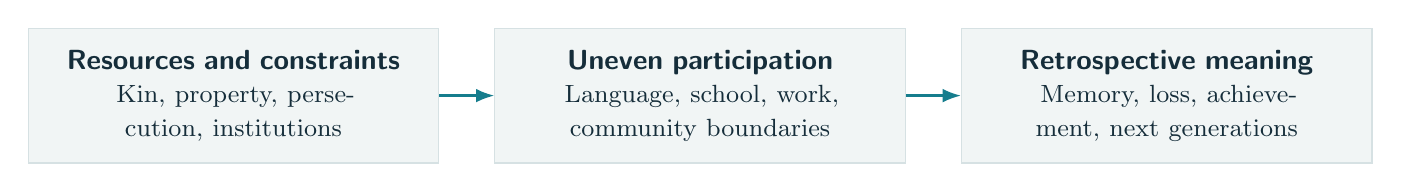
\begin{tikzpicture}[>=Latex,node distance=7mm,box/.style={draw=line,fill=paper,text width=4.65cm,minimum height=1.7cm,align=center,inner sep=8pt}]
\node[box] (a) {\sffamily\bfseries\color{ink}Resources and constraints\par\normalfont\small Kin, property, persecution, institutions};
\node[box,right=of a] (b) {\sffamily\bfseries\color{ink}Uneven participation\par\normalfont\small Language, school, work, community boundaries};
\node[box,right=of b] (c) {\sffamily\bfseries\color{ink}Retrospective meaning\par\normalfont\small Memory, loss, achievement, next generations};
\draw[->,teal,thick] (a)--(b);\draw[->,teal,thick] (b)--(c);
\end{tikzpicture}
{\footnotesize\color{muted}Figure 2. Reviewer-proposed organising sequence for a future synthesis. Arrows show an analytic reading order, not demonstrated causal effects. This structure is not an output already agreed by the coders or produced by Aperture.}

The combined account would explain how resources and constraints shape possible routes, how settlement broadens participation unevenly, and how narrators later weigh what migration cost against what it enabled. Partial childhood memory qualifies every stage: absence of recall cannot be automatically filled with a causal story about trauma or deliberate concealment.

\textbf{What should not be claimed.} The supplied artifacts do not establish that the AI lacks the ability to form overarching themes, that its different structure is a failure, or that a human four-theme structure is inherently superior. They establish a specific comparative weakness in this export's integration of long-term meaning.
\source{Machine \texttt{corpus\_level.json}, ``what the material shows'' and ``what this may mean''; consolidated overarching rows 1--4; all three final human overarching sheets.}

\page{09 / PASSAGE REVIEW}{Read overlap as a set of meanings}
\begin{takeaway}
\textbf{Review coverage.} The two Terra reviewers were assigned all 267 consolidated rows, all eight interviews, the corresponding original human records and all 985 AI claims. The lead read the calibration record and thematic narratives, inspected the returned judgments, and reopened contested evidence. The combined ledger records each row's interpretation, reasons and claim references.
\end{takeaway}

\subsection*{Three recurring relationships}
\begin{tabularx}{\linewidth}{@{}p{3.2cm}YY@{}}
\toprule
\textbf{Relationship} & \textbf{Example} & \textbf{What the comparison establishes}\tabularnewline\midrule
Same meaning, different names & T4 clan membership: cultural connection/preservation/traditions; AI organised Scottish meetings, dance and bagpipes. & Different labels can identify a common cultural-maintenance pattern. The book's divergence designation should not override that reading.\tabularnewline\addlinespace
Same passage, incomplete meaning & T6 the trunk and bundle containing all worldly goods; AI tracks the mother's management of children and luggage. & Practical caregiving is present, but material reduction to portable possessions needs a separate reading. A passage match does not establish completeness.\tabularnewline\addlinespace
Same meaning, different passage anchor & T3 a feverish infant removed from his mother; AI records the removal, uncertainty, three-day wait and reunion in several claims. & An unlinked human row can be substantively represented elsewhere in the same interview's AI analysis.\tabularnewline\bottomrule
\end{tabularx}

\subsection*{What the missed material adds}
Some residual omissions are consequential: Kaiz's derivative citizenship account makes legal dependence visible; severe journey illness adds embodied cost; housing without running water adds ordinary settlement deprivation; retrospective statements about childhood work can turn a list of chores into a life-course interpretation. These have different analytical value and should not each count as one identical ``miss.''

\subsection*{What the additional AI material adds}
Much of the unaligned AI material expands context rather than introducing a wholly new theme. The most useful contributions connect details: Larsen's furniture apprenticeship supplies blueprint skills for contracting; Thome's boarders and later rental flats reveal a changing household economy; Rizzuto's workplace exits connect wages and asserted freedom to an eventual restriction on mobility. Other claims merely subdivide a known episode. No overall novelty or precision rate is estimated for the 570 AI-only claims.

\begin{caution}
\textbf{The review required correction too.} Lead checks found that initial subagent judgments had mistaken missing lexical links for absent interpretations in several cases. Those judgments were reopened against the full claim inventory. This is why the report leads with inspectable cases and qualified comparative findings, rather than converting the ledger into a benchmark accuracy percentage.
\end{caution}
\source{Crosswalk rows 68, 100, 176; T1 derivative citizenship and journey illness; T8 housing; AI local craft, lodging and workplace themes. The ledger is a descriptive audit of model judgments, not independent human agreement.}

\page{10 / CLOSE-READING CASES}{Genuine omissions beside substantive recovery}
\case{T1 / Embodied transit costs remain underdeveloped}
{C1's ``Physical difficulties'' and C2/C3's physical-toll/difficult-journey readings are supported by severe sickness; a longer excerpt also includes a train-door hand injury. The meeting explicitly agrees on the shared hardship meaning.}
{The T1 claim set does not develop that sickness/injury experience. Claims about violence, separation and institutional vulnerability do not substitute for bodily suffering in transit. This is a supported omission. Rows 11 and 27 overlap, however, so they are not two independent missed events.}
{T1 source illness account; crosswalk rows 11 and 27; calibration lines 9--98; original human excerpts.}

\case{T1 / Legal dependency is a distinct human contribution}
{C2 codes ``Dependent legal status'' where Kaiz describes citizenship obtained through her father or husband. This makes a legal and gendered relationship visible.}
{No corresponding T1 AI claim develops derivative citizenship. Its household-authority theme does not capture this institutional relationship. This finding concerns what the narrator reports; the historical legal rule itself was not independently verified.}
{T1 opening citizenship account; crosswalk row 3; C2 initial code and explanation.}

\case{T2 / The AI does capture lasting distress}
{The narrator relates being under a train seat, dust and fear of suffocation to subsequent intolerance of enclosed spaces. Human trauma/lasting-impact codes are warranted as readings of her account.}
{The AI's ``Children's journey as freedom and ordeal'' explicitly preserves the enduring consequence, S297. This challenges the calibration's prediction that AI would necessarily miss such implicit trauma. It does not validate a clinical diagnosis or establish causation beyond the narrator's attribution.}
{T2 train journey; crosswalk row 46; AI local journey claim 7, S297; calibration at 1:17:11.}

\case{T3 / A lexical nonmatch is not an analytical absence}
{The mother spends three terrible days after officials take her feverish nursing infant. Human meanings include separation, health barriers and fear.}
{Aperture represents removal without explanation, fear of return, prolonged uncertainty, recovery and the mother's relief. Claims under family separation and the child's threshold jointly preserve the human meanings despite the row's missing lexical link.}
{Crosswalk row 68; AI T3 family-separation claims 9--11, S150--S153; child's-threshold claims 3--9; emotional-weight claims 2--3.}

\page{11 / INTERPRETIVE WARRANT}{Where the AI's explanation needs revision}
\case{Batta was 24 on arrival, not a child}
{T7's source header states birth in 1897 and arrival in 1921, ``AGE 24.'' The interview confirms the birth year. Her father left when she was three, but the eventual Ellis Island encounter occurred in adulthood.}
{The AI groups 14 T7 arrival/detention claims under ``Ellis Island as a child's threshold'' and treats meeting her unfamiliar father within a childhood-memory narrative. The individual events can be sound while the thematic developmental frame is wrong. Revise the scope to include adult arrival or explicitly separate Batta as a contrasting case.}
{T7 source lines 8--21 and 37--39; AI T7 child's-threshold block; childhood-memory claim 7, S311; family-separation claim 1 explicitly acknowledges adulthood.}

\case{Friedman's volunteering: bereavement, reciprocity and conjecture}
{C2's ``Volunteering as healing'' is supported in context: after her husband's death she felt lost, volunteered more, and says the work did a great deal for her. C1 also sees giving back to migrants.}
{Aperture captures translation, retained Russian, later service and personal benefit. Its theme title goes further: absence of arrival support \emph{prompting} volunteerism. The interviewer juxtaposes her service with the help her family lacked, but she does not directly identify that absence as the cause of her volunteering. Bereavement is the more explicit trigger. Retain the reparative interpretation as a hypothesis, not an established mechanism.}
{T5 source lines 218--236; crosswalk row 158; AI local volunteerism claims 2, 7 and 12, S522/S533/S551; theme definition.}

\case{A household economy is more than a list of tasks}
{Thome's human codes connect long hours, childhood chores, family responsibility and hardship. Some retrospective loss-of-childhood meaning remains less explicit in the AI.}
{The AI adds a concrete account: sixteen boarders, food rather than wages for the mother's labour, reliance on boarding when the father cannot work, and a later shift to rental income. This has analytical value. Yet causal shorthand in summaries and claims needs checking; a detailed ledger does not guarantee that every explanatory connection is supported.}
{T6 source boarding/work accounts; crosswalk rows 168, 173, 180, 185, 207--208; AI lodging claims 3, 7--8, 11--14; children's-household-labour claims 3--10.}

\begin{takeaway}
\textbf{The main risk is not merely hallucinated facts.} It is the movement from a supported event to a too-broad organising claim: adult experience becomes childhood experience; later service becomes a causal repair of earlier neglect; multiple local trajectories become a universal story. Human interpretations require the same scrutiny.
\end{takeaway}


\page{12 / OVERALL ASSESSMENT}{A capable analytic partner, with evidence checks}
\begin{tabularx}{\linewidth}{@{}p{3.2cm}Y@{}}
\toprule
\textbf{Dimension} & \textbf{Judgment from this corpus}\tabularnewline\midrule
Human--human comparison & Considerable shared meaning coexists with selection differences and different levels of abstraction. The workbook's divergence labels overstate substantive opposition in demonstrated cases. A corrected population agreement rate is not established.\tabularnewline
Adjudication contribution & Strongest when it exposes assumptions and improves boundaries; weaker when assent substitutes for checking the source. Its religion error shows why a consensus reference requires an evidence audit.\tabularnewline
AI evidentiary contribution & Detailed traceable propositions, alternative organising ideas and concrete economic/social mechanisms. Evidence links and caveats help review, but local paraphrase and causal expansion can still be mistaken.\tabularnewline
AI thematic contribution & Substantial overlap with most consolidated comparison dimensions, plus explicit attention to mediation, property/class and enclave limits. Long-term/intergenerational meaning is less integrated in the corpus explanation.\tabularnewline
Relative strengths & C1 contributes a differentiated architecture and reflective questions; C2 foregrounds temporal and intergenerational meaning; C3 preserves practical distinctions; the AI supplies granular mechanisms and an alternative memory-centred synthesis. None is uniformly best across all tasks.\tabularnewline\bottomrule
\end{tabularx}

\subsection*{Changes warranted in the evaluation package}
Replace ``near-zero agreement'' with the actual descriptive verdict counts and a warning that these are not reliability scores. Mark the 9+4 patterns as \emph{consolidated comparison dimensions}, with links to what was and was not resolved in the session. Correct the T7 identity note. Retain the lexical alignment strictly as a navigation aid. Describe AI overarching output as ``no named tier; corpus-level synthesis present.'' Keep final human theme passes distinct from drafts.

\subsection*{Changes warranted in Aperture's output}
First, require qualified actor and mechanism claims: who felt what, which evidence supports the causal link, and what remains uncertain? Second, repair downstream summaries after claims are removed; the Friedman local summary explicitly says it predates a dropped claim. Third, qualify apparent corpus-wide patterns with mixed or contrary cases. Fourth, distinguish ``not examined'' from ``not found.'' Finally, develop a short synthesis connecting local trajectories to long-term consequences, with reasons for each grouping and visible alternatives.

\begin{takeaway}
\textbf{Decision.} Use this AI export as a substantive additional analysis and a source of hypotheses for comparison. The evidence supports a collaborative workflow with direct source checks. It does not support declaring either the human consensus or the AI output an authoritative ground truth, or assigning an overall percentage of ``human-level coding.''
\end{takeaway}

\page{13 / NEXT VALIDATION DESIGN}{Turn this audit into a defensible benchmark}
\textbf{1. Fix the analytic brief before rerunning.} Choose a research question, intended level of abstraction and output budget shared by human and AI conditions. Record theory exposure, iteration opportunities and whether the goal is reflexive interpretation or a predefined coding task. Run these as separate study designs if both are wanted.

\textbf{2. Separate reference construction from candidate evaluation.} Build passage dossiers from the whole corpus, including passages selected by neither side. Have researchers describe multiple defensible meanings and known limits before seeing attributed human/AI outputs. This avoids rewarding either side simply because its selections define the evaluation universe.

\textbf{3. Compare anonymised propositions, then restore the thematic context.} Review fidelity and inferential warrant first with provenance masked where feasible. Next examine complete thematic structures for organising concepts, boundaries, negative cases and explanatory value. Keep evidence quality separate from stylistic fluency and output length.

\textbf{4. Audit the exceptional cases completely.} Revisit all 59 lexical nonmatches and all disputed source/identity or causal claims identified here. For the 570 AI-only claims, deduplicate by episode and stratify by transcript, theme and caveat status. Judge added value, redundancy and unsupported extension separately; do not label everything ``novel.'' Inspect additional source passages outside both selections to study shared omissions.

\textbf{5. Use independent researchers for consequential judgments.} Obtain two qualitative researchers' written reasons on the same cases, including all proposed substantive errors. A third can resolve factual disputes and document interpretive alternatives. If the future design is reflexive TA, report the reflexive differences rather than turning agreement into a universal quality criterion.

\textbf{6. Test robustness rather than one export.} Repeat the AI analysis with documented settings and controlled prompts, and compare interpretation stability across runs. Evaluate other corpora and research questions before generalising. Measure time or cost only in a prospectively matched workflow.

\subsection*{What this report does and does not establish}
\begin{tabularx}{\linewidth}{@{}YY@{}}
\toprule
\textbf{Established here} & \textbf{Still unestablished}\tabularnewline\midrule
An evidence-based comparison of supplied meanings and structures; concrete human, adjudication and AI weaknesses; a traceable row-level review; corrections to misleading package claims. & Population accuracy, recall, inter-rater reliability, causal determinants of migrant outcomes, performance on unseen corpora, and relative time/cost efficiency.\tabularnewline\bottomrule
\end{tabularx}

\begin{caution}
\textbf{Reviewer limitation.} The passage reviews and final synthesis were produced by language models. Transcript assignments were divided between Terra subagents, not independently double-coded in full. The lead performed additional source checks and reviewed the returned reasoning. These shared model-based judgments may have correlated blind spots; the ledger is an audit trail, not human validation.
\end{caution}

\page{14 / EVIDENCE AND REPRODUCIBILITY}{Read the report; inspect the decisions}
\subsection*{Supplied evidence}
\begin{tabularx}{\linewidth}{@{}p{4.2cm}Y@{}}
\toprule
\textbf{Locator used in this report} & \textbf{Source in the evaluation package}\tabularnewline\midrule
T1--T8 and line numbers & \texttt{sources/T1.txt} through \texttt{T8.txt}: Kaiz, Larsen, Turkin, Hansen, Friedman, Thome, Batta, Rizzuto. These are source accounts, not independently verified historical facts.\tabularnewline
Crosswalk row N & \texttt{crosswalk/segment\_alignment.json}; stable global row field, 1--267. Includes consolidated codes and lexical AI links.\tabularnewline
Human books & \texttt{human/c1\_nirosha.json}, \texttt{c2\_arnisha.json}, \texttt{c3\_bohdan.json}. C3 is Karolina Joanna Bohdan.\tabularnewline
Consolidated patterns & \texttt{adjudication/consolidated.json}; nine candidate comparison rows and four overarching comparison rows.\tabularnewline
Calibration & \texttt{adjudication/calibration\_session.md}; full 81-minute ASR record. \texttt{calibration\_index.json} is a preparer's guide, not independent confirmation.\tabularnewline
AI claim / theme / passage & \texttt{machine/claims.json}, \texttt{themes.json}, \texttt{materials.json}. Passage IDs repeat by interview; always retain transcript and theme. Exact claim IDs appear in the accompanying ledger.\tabularnewline
AI synthesis / process & \texttt{machine/corpus\_level.json}; narratives, open questions, exclusions, feedback status and processing history.\tabularnewline\bottomrule
\end{tabularx}

\subsection*{Evaluation deliverables}
\texttt{evaluation.pdf} is the rendered report; \texttt{evaluation.tex} and \texttt{passage\_results.tex} are the editable LaTeX sources. The \texttt{review/} folder contains the two transcript-review ledgers and syntheses, the combined review, the lead's checks, descriptive statistics and a SHA-256 input manifest. The companion README explains how to navigate and rebuild the report.

No regex, string-similarity threshold or embedding similarity was used to decide interpretive agreement in this review. Scripts were used to organise evidence, verify identifiers and counts, generate tables and compile the document. The pre-existing lexical crosswalk was treated as retrieval metadata only.

\subsection*{Methodological references}
Braun, V., and Clarke, V. \emph{Got questions about thematic analysis?} Author-maintained FAQ, especially the discussions of multiple coders, interpretive quality and reflexive collaboration. Accessed 6 September 2026. \url{https://www.thematicanalysis.net/faqs/}

Braun, V., and Clarke, V. \emph{Evaluating and reviewing (reflexive) TA research: A guide for editors and reviewers.} Author-maintained guidance on methodological coherence and themes as shared meaning. Accessed 6 September 2026. \url{https://www.thematicanalysis.net/editor-checklist/}

{\footnotesize\color{muted}Berry and Portes are discussed as theoretical influences reported by the coders. Their original works were not reviewed for this audit; no finding here validates the coders' representations of those theories. The primary evidentiary basis of the comparison is the supplied interview and coding record.}
\end{document}
